% THIS DOCUMENT IS FOLLOWS THE VOLERE TEMPLATE BY Suzanne Robertson and James Robertson
% ONLY THE SECTION HEADINGS ARE PROVIDED
%
% Initial draft from https://github.com/Dieblich/volere
%
% Risks are removed because they are covered by the Hazard Analysis
\documentclass[12pt]{article}
\usepackage{graphicx}
\usepackage{float}
\usepackage{parskip}
\usepackage{xcolor} 

\usepackage{booktabs}
\usepackage{tabularx}
\usepackage{hyperref}
\hypersetup{
    bookmarks=true,         % show bookmarks bar?
      colorlinks=true,      % false: boxed links; true: colored links
    linkcolor=red,          % color of internal links (change box color with linkbordercolor)
    citecolor=green,        % color of links to bibliography
    filecolor=magenta,      % color of file links
    urlcolor=cyan           % color of external links
}

\newcommand{\lips}{\textit{Insert your content here.}}

% %% Comments

\usepackage{color}

\newif\ifcomments\commentstrue %displays comments
%\newif\ifcomments\commentsfalse %so that comments do not display

\ifcomments
\newcommand{\authornote}[3]{\textcolor{#1}{[#3 ---#2]}}
\newcommand{\todo}[1]{\textcolor{red}{[TODO: #1]}}
\else
\newcommand{\authornote}[3]{}
\newcommand{\todo}[1]{}
\fi

\newcommand{\wss}[1]{\authornote{blue}{SS}{#1}} 
\newcommand{\plt}[1]{\authornote{magenta}{TPLT}{#1}} %For explanation of the template
\newcommand{\an}[1]{\authornote{cyan}{Author}{#1}}

% %% Common Parts

\newcommand{\progname}{Scanalyze AI} % PUT YOUR PROGRAM NAME HERE
\newcommand{\authname}{Team 16, Ace
\\ Hamza Issa
\\ Ahmad Hamadi
\\ Jared Paul
\\ Gurnoor Bal} % AUTHOR NAMES                  

\usepackage{hyperref}
    \hypersetup{colorlinks=true, linkcolor=blue, citecolor=blue, filecolor=blue,
                urlcolor=blue, unicode=false}
    \urlstyle{same}
                                


\begin{document}

\title{Software Requirements Specification for \progname: subtitle describing software} 
\author{\authname}
\date{\today}
	
\maketitle

~\newpage

\pagenumbering{roman}

\tableofcontents

~\newpage

\section*{Revision History}

\begin{tabularx}{\textwidth}{p{3cm}p{2cm}X}
\toprule {\textbf{Date}} & {Author} & {Section}\\
\midrule
11 October 2024 & Ahmed & 7-9, 24-26 \\
11 October 2024 & Harrison & 18-23 \\
11 October 2024 & Jared & 1-2, 15-17 \\
11 October 2024 & Hamza & 10-15 \\
11 October 2024 & Gurnoor & 3-6 \\
\bottomrule
\end{tabularx}

~\\

~\newpage
\section{Purpose of the Project}

\textbf{Current Content:} The document currently describes an AI tool for analyzing chest X-rays, focusing on assisting radiologists with diagnostic reports.  \\
\\
{\textcolor{blue}{Update Needed:}} We need to revise this section to clearly state that our project is now focused on developing a \textbf{multi-class classification CNN model} that can categorize chest X-ray images into multiple disease types (e.g., pneumonia, tuberculosis, cardiomegaly, normal, etc.). Instead of simply enhancing efficiency for radiologists, our system aims to \textbf{automate and improve the accuracy of chest X-ray disease classification}, providing a structured and interpretable output.\\

\subsection{User Business}
Chest X-rays are essential to the healthcare industry for diagnosing lung and heart conditions. 
However, the interpretation of these images are complex and require a high level of expertise. 
This project intends to tackle this challenge by creating an ai diagnostic tool that analyzes 
chest x-rays and generates medical reports, enhancing efficiency and accuracy in diagnosis. The 
development of this diagnostic tool will lead to the enhancement of patient care and the 
efficiency of the medical industry. 

\subsection{Goals of the Project}
\textbf{Current Content:} The SRS describes a tool that enhances efficiency and accuracy in diagnosis by generating structured reports. \\
\\
{\textcolor{blue}{Update Needed:}} This section should now emphasize our \textbf{multi-class nature of disease classification}, including defining key performance indicators such as \textbf{precision, recall, F1-score, confusion matrices, and AUC-ROC scores} to evaluate our model. The goal should also shift from merely assisting radiologists to \textbf{developing an independent AI-based classification system} that can be integrated into medical workflows.\\

The objective of this project is to create a neural network model that can precisely analyze chest 
X-rays and produce diagnostic reports to help radiologists diagnose heart and lung diseases. By 
using this tool, radiologists' workload will be reduced, diagnostic accuracy will increase, and 
workflow efficiency will be improved—all of which will improve patient care. The model's capacity 
to identify diseases with a high degree of accuracy and to drastically cut down on the time and 
effort required for radiologists to generate reports will determine its success. The tool's 
usefulness and efficacy will be assessed using performance metrics and radiologists' input.

\section{Stakeholders}

\textbf{Current Content:} Mentions radiologists, biomedical researchers, AI researchers, and hospitals as key stakeholders. \\
\\
{\textcolor{blue}{Update Needed:}} While stakeholders remain the same, the shift in project focus means that \textbf{medical AI researchers and data scientists} will play a bigger role in validating the classification model. Additionally, \textbf{hospitals and healthcare institutions} that may integrate this model for \textbf{real-time disease detection} should be included as key stakeholders.\\

\subsection{Client}
\textbf{Medical Technology Department and/or healthcare organization sponsoring the initiative: }
This client is responsible for funding and overseeing the progress of the project to ensure it 
meets their objectives.

\subsection{Customer}
\textbf{Radiologists and Medical Imaging Specialists: } Use the system to interpret chest X-rays 
more effectively, providing input on system performance and ensuring alignment with diagnostic 
procedures.

\textbf{Healthcare Institutions: } Implement the technology to improve patient care by delivering 
faster and more accurate chest X-ray results.

\textbf{Patients: } Benefit from quicker and equally accurate X-ray results, leading to an 
improved treatment experience.

\subsection{Other Stakeholders}
\textbf{Healthcare Administrators: } Oversee the implementation of the system in clinical settings 
and ensure compliance with medical standards and regulations.

\textbf{Biomedical and AI Researchers: } Researchers interested in the intersection of AI and 
healthcare who will benefit from new research insights and may conduct their own studies based on 
this project.

\textbf{Hospitals and Medical Centers:} Institutions that will implement this technology for 
faster and more accurate diagnoses.

\subsection{Hands-On Users of the Project}

\textbf{Radiologists}
\begin{itemize}
    \item {\textbf{User Role: } Diagnose patients based on chest X-ray analysis.}
    \item {
        \textbf{Experience in Subject Matter: } Radiologists have a great deal of expertise 
        regarding diagnostic procedures and medical imaging. They know how to analyze results from
         a variety of imaging modalities and comprehend how discoveries may have therapeutic 
        ramifications.
    }
    \item {
        \textbf{Technological Experience: } Well-versed in imaging technologies, diagnostic software, and instruments with artificial intelligence. They frequently adjust to new systems that improve workflow.
    }
\end{itemize}

\textbf{Medical Technologists}
\begin{itemize}
    \item {\textbf{User Role: } Operate imaging equipment and assist in diagnosis}
    \item {
        \textbf{Subject Matter Experience: } Medical technologists have a solid understanding 
        of the technology and the science behind imaging procedures.
    }
    \item {
        \textbf{Technological Experience: } Proficient in operating imaging devices and related 
        software, allowing them to efficiently gather and process imaging data.
    }
\end{itemize}

\textbf{Nurses}
\begin{itemize}
    \item {\textbf{User Role: } Assist in patient care and manage patient records.}
    \item {
        \textbf{Subject Matter Experience: } Nurses are knowledgeable about patient care protocols
         and the importance of imaging in diagnostics. They understand how imaging impacts 
         treatment decisions.
    }
    \item {
        \textbf{Technological Experience: } Familiar with electronic health record (EHR) systems 
        and patient management software but may have limited exposure to advanced imaging 
        technologies.
    }
\end{itemize}

\textbf{Patients}
\begin{itemize}
    \item {\textbf{User Role: } Individuals receiving chest X-ray services.}
    \item {
        \textbf{Subject Matter Experience: } Patients may have varying degrees of understanding 
        regarding medical imaging and its implications for their health, often informed by prior 
        experiences or education.
    }
    \item {
        \textbf{Technological Experience: } Generally limited technological experience with 
        medical systems; they typically interact with healthcare technology through appointments 
        and diagnostic processes
    }
\end{itemize}

\subsection{Personas}
\textbf{Dr. Emily Richards} is a 47-year-old radiologist working at a local hospital. Emily is 
married with two children, who are of age 8 and 12. Some of her hobbies include going on walks and 
hikes. She also enjoys reading which ranges from fictional novels to medical journals. She lives 
in a suburban area right outside a major city. Emily has a passion for Italian cuisine, 
particularly pasta, and enjoys classic rock, though she switches to classical music while working 
in her office. Her favourite holiday destination is going to Florida to visit her mom and dad, 
where she enjoys spending quality time with family and relaxing in the sun. She dislikes not being 
up to date with the latest technology and feeling stagnant in her learning and professional 
development. Dr. Richards is open to new technology, believing it can enhance patient care and can 
make her more efficient at her job. She is cautious about spending but willing to invest in tools 
that significantly improve her productivity or patient care outcomes. She believes that our X-ray 
model represents a significant advancement in her field, aligning with her interests in 
technological innovations and improvements in efficiency.

\subsection{Priorities Assigned to Users}
\textbf{Key Users:}
\begin{itemize}
    \item{
        \textbf{Radiologists: } Critical to the success of the AI system, as they will rely on 
        it for diagnostic assistance. Their feedback will shape the usability and functionality of 
        the product.
    }
    \item {
        \textbf{Medical Imaging Specialists: } Essential for ensuring the correct interpretation 
        of X-rays and validation of medical reports. Their expertise influences the model's 
        accuracy and performance.
    }
\end{itemize}

\noindent
\textbf{Secondary Users:}
\begin{itemize}
    \item{
        \textbf{Patients: } While they benefit from the product's outcomes, their direct feedback 
        may not significantly impact its design or success. Their needs are considered but are 
        secondary to those of the key users.
    }
\end{itemize}

\subsection{User Participation}
\textbf{Radiologists: } Provide insights on diagnostic workflows and usability requirements. \\
Estimated time: 10 hours for feedback sessions and testing.
\\
\noindent
\textbf{Medical Imaging Specialists: }Offer expertise in interpreting medical images and 
validating AI outputs. \\
Estimated time: 8 hours for reviews and discussions.
\\
\noindent
\textbf{Patients:} Share feedback on their experiences and expectations regarding chest X-ray 
results. \\
Estimated time: 4 hours for surveys or focus groups.
\\
\noindent
\textbf{AI Researchers and Engineers:} Contribute technical knowledge on AI applications and 
assist in interface prototyping. \\
Estimated time: 6 hours for collaborative development sessions.


\subsection{Maintenance Users and Service Technicians}
Radiology Support Specialist: Focuses on maintaining and troubleshooting the AI system used in 
radiology departments.
\\
\noindent
Clinical Systems Technician: Works on the upkeep and repair of clinical technology systems, 
including the AI product.
\\
\noindent
AI Systems Maintenance Engineer: Responsible for the ongoing support and maintenance of AI-driven 
diagnostic tools.

\section{Mandated Constraints}

\textbf{Current Content:} The document currently lists general project constraints. \\
\\
\textbf{\textcolor{blue}{Update Needed:}} Include constraints related to \textbf{dataset quality, model accuracy thresholds, and regulatory compliance (HIPAA, GDPR)}. Define \textbf{minimum expected classification accuracy} and processing time constraints for real-world deployment.


This section defines the essential requirements the product must follow, including legal, 
regulatory, or system-related restrictions. These constraints ensure the product complies with 
necessary standards and functions within the project's limitations.

\subsection{Solution Constraints}
This subsection outlines the constraints placed on the proposed solution for the chest X-ray 
analysis project. These constraints cover the technical environment, supporting systems, workplace 
and enterprise considerations, as well as the fit criteria required for each.
\\\\
\indent
MC1: The product shall operate as a web application

Rationale: The web-based nature of the system will allow medical professionals, researchers, and 
other stakeholders to access the system easily across various platforms (Windows, MacOS, Linux, 
etc.) without requiring complex local installations.

Fit Criterion: The product will include back-end, front-end, and database integration to run as a 
web application accessible via a URL, optimized for different devices and browser types (Chrome, 
Firefox, Safari, etc.).
\\\\
\indent
MC2: The product shall integrate publicly available chest X-ray datasets (CheXpert, MIMIC)

Rationale: Using public datasets will ensure that the project has access to a broad range of chest 
X-ray images needed for training and testing the neural network without violating patient privacy 
laws.

Fit Criterion: The solution will successfully use the CheXpert and MIMIC datasets for model 
training, with scripts to download and preprocess these datasets for CNN usage. It will comply 
with healthcare privacy standards (e.g., HIPAA).

\subsection{Implementation Environment of the Current System}
This section outlines the technological and physical environment in which the product will be 
installed and operated. It encompasses all relevant hardware, software, and organizational 
elements that will interact with the system. The goal is to provide a comprehensive understanding 
of the current infrastructure so that the product can be designed to effectively integrate and 
function within this environment. Understanding the operational requirements derived from this 
description will help the design team ensure that the solution meets all necessary criteria for 
successful implementation and usability in real-world settings.
\\\\
\noindent
MC3. The product shall use machine learning frameworks like TensorFlow or PyTorch

Rationale: Machine learning frameworks are essential for training the convolutional neural network 
(CNN) model. TensorFlow and PyTorch are widely used, industry-standard frameworks that offer 
extensive support for neural network development and GPU acceleration.

Fit Criterion: The product will use either TensorFlow or PyTorch for model development and 
training, with support for cloud-based GPU instances to speed up computation.

\subsection{Partner or Collaborative Applications}
This section identifies and describes systems external to the product but necessary for its 
operation and integration. These systems may include internal databases, external software 
solutions, or third-party services. Understanding these relationships is essential for ensuring 
smooth integration and efficient product functionality within the broader technological 
environment.
\\\\
\noindent
MC4. The product shall integrate with external healthcare information systems.

Rationale: These systems are essential for accessing and managing patient data, facilitating 
seamless communication between the product and existing infrastructures. Integrating with these 
systems will enhance the product's ability to deliver accurate results within the clinical 
workflow.

Fit Criterion: The product will support integration with healthcare systems through standardized

\subsection{Off-the-Shelf Software}
This section identifies and describes commercial, open-source, and other off-the-shelf software 
(OTS) products that will be incorporated into the solution. The use of OTS software is intended to 
leverage existing capabilities and minimize development time. Understanding the characteristics, 
behaviors, and interfaces of these products will help define the design constraints and inform 
decision-making throughout the project lifecycle. Additionally, potential conflicts between the 
requirements and the capabilities of the OTS software must be considered to ensure that the 
product aligns with organizational needs.
\\\\
\noindent
MC5. The product shall integrate with a commercial machine learning framework

Rationale: Established frameworks like TensorFlow or PyTorch provide robust tools for developing 
and training machine learning models, allowing for efficient implementation of advanced algorithms.

Fit Criterion: The product will utilize the selected framework to train and deploy convolutional 
neural networks for analyzing chest X-ray images, ensuring compliance with model performance 
benchmarks.


\subsection{Anticipated Workplace Environment}
This section outlines the anticipated workplace environment where users will interact with the 
product. Understanding the features of this environment is critical for ensuring that the product 
is designed effectively to meet user needs and to compensate for any potential difficulties. The 
description will encompass physical aspects, such as space layout and equipment, as well as social 
and cultural factors that may impact the product's usability and acceptance.
\\\\
\noindent
MC6. The product is intended for use in healthcare settings

Rationale: Working in healthcare environments imposes strict regulations and standards for data 
security and patient privacy, which must be considered in the product design.

Fit Criterion: The product will implement robust security measures, including encryption and 
access controls, to ensure compliance with healthcare regulations and protect sensitive patient 
information.


\subsection{Schedule Constraints}
This section outlines the critical timelines and deadlines associated with the project’s 
development phases. Establishing a clear schedule is essential for managing resources, 
coordinating team efforts, and ensuring that all project components are delivered on time. These 
constraints help prioritize tasks and guide decision-making throughout the project lifecycle, 
ultimately contributing to the successful implementation of the proposed solution. By identifying 
key milestones, this section clarifies the expectations for progress and accountability, enabling 
the team to meet operational and stakeholder requirements efficiently.
\\\\
\noindent
MC7. The key milestones of the project’s proposed solution must be completed by specified 
deadlines.

Rationale: This ensures that each major phase of the project is delivered on time, allowing 
sufficient opportunities for testing, evaluation, and any necessary adjustments before the final 
release. Timely completion is critical for aligning with external dependencies and operational 
readiness.

Fit Criterion: All significant milestones, including the completion of the proof of concept, 
initial version, and final version demonstrations, must adhere to the following schedule:\\
Proof of Concept Demonstration to occur between November 11 - 22, 2024\\
Revision 0 Demonstration to take place between February 3 - 14, 2025\\
Final/Revision 1 Demonstration scheduled for March 24 - 30, 2025\\
Final/Revision 1 Documentation scheduled for April 2, 2025\\


\subsection{Budget Constraints}
This section outlines the financial limitations associated with the project, detailing the budget 
allocated for developing the proposed solution. It emphasizes the necessity for cost-effective 
planning and resource allocation to ensure that the project remains within its financial 
boundaries.
\\\\
\noindent
MC8. The total budget for the project’s proposed solution is limited to \$750

Rationale: This budgetary limit is established to prevent the acquisition of pre-existing 
solutions and to promote the development of a tailored solution. It emphasizes the importance of 
minimizing all associated costs to maintain financial efficiency throughout the project.

Fit Criterion: The combined expenses for all necessary hardware and software to execute the 
project’s proposed solution must not exceed \$750.

\subsection{Enterprise Constraints}
N/A

\section{Naming Conventions and Terminology}
\subsection{Glossary of All Terms, Including Acronyms, Used by Stakeholders
involved in the Project}
Motivation: Names are very important. They invoke meanings that, if carefully defined, can save 
hours of explanations. Attention to names early in the project helps to highlight 
misunderstandings. As the detailed work progresses, the glossary provides input to the more 
precisely specified business/work data model and data dictionary.

Glossary of All Terms, Including Acronyms, Used By Stakeholders\\

\textbf{ML}:\\
Machine Learning: A branch of artificial intelligence that involves the use of algorithms to allow 
computers to learn from and make predictions based on data. This is a core technology used in the 
project for analyzing chest X-rays.

\textbf{DL}:\\
Deep Learning: A subset of machine learning involving neural networks with many layers, used to 
analyze various types of data, including images.

\textbf{DICOM}:\\
Digital Imaging and Communications in Medicine: A standard for transmitting, storing, and sharing 
medical imaging information. It is used to manage medical images in the proposed solution.

\textbf{CNN}:\\
Convolutional Neural Network: A type of deep learning model specifically designed for processing 
structured grid data like images, used in the project for chest X-ray analysis.

\textbf{EHR}:\\
Electronic Health Record: A digital version of a patient's paper chart, used for storing patient 
information and history that may be integrated with the proposed solution.

\textbf{API}:\\
Application Programming Interface: A set of rules and protocols for building and interacting with 
software applications, enabling the integration of the proposed solution with other systems.

\textbf{MC}:\\
Mandated Constraints: Various constraints placed on the project’s proposed solution that must be 
adhered to throughout the development process.

\textbf{FR}:\\
Functional Requirement: A requirement that specifies what functionality the project’s proposed 
solution must provide to meet user needs.

\textbf{NFR}:\\
Nonfunctional Requirement: A requirement that specifies criteria that can be used to judge the 
operation of a system, rather than specific behaviors (e.g., performance, usability).

\textbf{BUC}:\\
Business Use Case: A scenario that describes how the proposed solution can be used within a 
business context to achieve specific goals.

\textbf{PUC}:\\
Product Use Case: A scenario that details how an individual user will interact with the proposed 
solution to achieve specific tasks.

\textbf{MVP}:\\
Minimum Viable Product: A version of the proposed solution that includes only the essential 
features required to meet the core needs of the users and stakeholders.

\section{Relevant Facts And Assumptions}
\textbf{Current Content:} Covers dataset availability, user expertise, and model reliability assumptions. \\
\\
\textbf{\textcolor{blue}{Update Needed:}} Modify to highlight \textbf{assumptions specific to multi-class classification}, such as \textbf{balanced datasets, diverse training samples, and real-world test set evaluation}. Address risks if \textbf{dataset bias is present or annotation errors exist}.

\subsection{Relevant Facts}

\textbf{Content:}\\
Relevant facts that affect the development of the proposed solution but are not specified as 
mandated requirements include the following:

Data Availability: A substantial dataset of annotated chest X-rays is available for training the 
machine learning model, facilitating effective learning and validation processes.

Technology Adoption: The target users (radiologists and medical technicians) are increasingly 
adopting AI-based tools in their workflow, indicating a positive reception and potential for 
successful implementation.

\textbf{Motivation:}\\
These relevant facts provide essential background information to stakeholders and development 
teams, helping them understand the business context in which the proposed solution will operate. 
They may also guide the formation of requirements as the project progresses and can impact design 
decisions to enhance user experience and regulatory compliance.

\subsection{Business Rules}
\textbf{Content:}\\
The following business rules have been identified that may impact the project related to chest 
X-ray analysis and the development of the proposed solution:

Patient Data Privacy: All patient data used for training and analysis must comply with HIPAA 
regulations, ensuring confidentiality and security in handling personal health information.

Reason for the Rule: To protect patient privacy and maintain legal compliance in the handling of 
sensitive information.

Authority for the Rule: Federal regulations and organizational policies governing health 
information.

Integration with EHR Systems: The solution must integrate seamlessly with existing Electronic 
Health Record (EHR) systems used by healthcare facilities.

Reason for the Rule: To facilitate workflow efficiency and ensure accurate patient record-keeping.
Authority for the Rule: Internal policies and standard practices in healthcare IT.

\textbf{Motivation:}\\
These business rules play a critical role in shaping the requirements for the proposed solution. 
By documenting and understanding these rules, the project team can ensure compliance and identify 
relevant requirements throughout the development process. Revisiting these rules as the project 
progresses will help maintain alignment with organizational and regulatory expectations.


\subsection{Assumptions}
The following assumptions have been made by the project team regarding the development and 
implementation of the chest X-ray analysis solution:

Availability of Training Data: It is assumed that sufficient high-quality, labeled chest X-ray 
images will be available for training the machine learning model.

Effect if False: If adequate training data is not available, the accuracy and reliability of the 
AI model may be compromised, potentially delaying the project timeline.

Technical Resources Availability: It is assumed that the necessary technical resources, including 
hardware and software tools, will be available on schedule for development and testing phases.

Effect if False: Delays in resource availability may lead to schedule slippage and affect overall 
project milestones.

\textbf{Motivation:}\\
By explicitly stating these assumptions, the project team aims to ensure all stakeholders are 
aware of the foundational beliefs guiding the project. Addressing these assumptions early helps 
manage expectations and facilitates proactive planning to mitigate risks associated with their 
potential inaccuracy.

\section{The Scope of the Work}

\textbf{Current Content:} Describes general project goals. \\
\\
\textbf{\textcolor{blue}{Update Needed:}} Revise to focus on \textbf{multi-class classification improvements}, including \textbf{disease differentiation accuracy and reducing misclassification rates}. Emphasize future \textbf{model adaptation to new disease categories}.

The scope of the work determines the boundaries of the business area to be studied and outlines 
how it fits into its environment. Our project, which focuses on AI-driven chest X-ray analysis, 
aims to create a convolutional neural network (CNN) model that assists radiologists in diagnosing 
lung and heart conditions. The boundaries of the work involve AI-driven diagnostics, healthcare 
applications, and web-based solutions for radiologists.

\subsection{The Current Situation}
The current diagnostic process for chest X-rays is primarily manual. Radiologists analyze images 
to detect abnormalities such as pneumonia, lung cancer, or cardiac conditions. While existing 
automated systems provide some assistance, they lack the accuracy and speed needed to fully 
integrate into a clinical workflow. Errors in diagnosis can occur due to the overwhelming number
of X-rays radiologists must process daily, contributing to diagnostic delays and potential 
misinterpretations. In the current environment, radiologists perform these tasks with limited AI 
assistance, and the process is often time-consuming and subject to human fatigue.

By improving AI-based diagnostic tools, the project aims to reduce the workload of radiologists 
and increase diagnostic accuracy. This involves replacing or augmenting manual processes with an 
advanced CNN model that can provide high-confidence predictions on chest X-rays. The study of the 
current situation allows us to understand the potential effects of such a change and select the 
most effective approach for integration.

The current process can be modeled using a swimlane diagram that outlines the roles of 
radiologists, existing software, and the proposed AI solution. The swimlane diagram would show the 
manual steps involved in diagnosing chest X-rays, including image acquisition, review by the 
radiologist, and final diagnosis, with clear points where automation via the CNN can intervene.


\subsection{The Context of the Work}
The work context diagram shows the interactions between the AI-driven chest X-ray diagnostic tool 
and other adjacent systems. Key external systems include the hospital's radiology information 
system (RIS), the picture archiving and communication system (PACS), and medical imaging databases 
like CheXpert or MIMIC. The product will take input from chest X-ray datasets or directly from 
hospital systems and provide diagnostic outputs to radiologists via a user interface.

Defining the work context helps ensure the AI diagnostic tool integrates seamlessly with existing 
hospital systems, avoiding any disruptions to current workflows. Without understanding these 
systems, the product might fail to meet critical requirements, such as compatibility with existing 
image formats or HIPAA compliance.

A context diagram can be used to map out the interaction between the chest X-ray diagnostic tool 
and the hospital’s RIS/PACS, showing the flow of X-ray data and diagnostic outputs. It would also 
include external AI model training systems and databases used for model validation.


\subsection{Work Partitioning}
The work can be divided into the following key business events, each representing a specific 
response in the diagnostic workflow. Each business use case (BUC) describes how the AI system will 
interact with the radiologists and adjacent systems:

Chest X-ray Image Upload
\begin{itemize}
    \item Input: X-ray images from the PACS system.
    \item Output: Pre-processed images ready for analysis by CNN.
    \item BUC Summary: The system ingests and processes the X-ray images, preparing them for 
        diagnostic analysis.
\end{itemize}

AI Diagnosis Processing
\begin{itemize}
    \item Input: Pre-processed chest X-rays.
    \item Output: Diagnostic predictions (lung or heart conditions).
    \item BUC Summary: The AI model analyzes the image and produces a diagnosis, complete with 
        confidence intervals and recommendations.
\end{itemize}

Radiologist Review
\begin{itemize}
    \item Input: AI-generated diagnosis.
    \item Output: Final diagnosis by radiologist, potentially informed or confirmed by the AI’s 
        findings.
    \item BUC Summary: The radiologist reviews the AI predictions and confirms the final 
        diagnosis, using the tool as an aid rather than a replacement.
\end{itemize}

Data Validation and Training Feedback
\begin{itemize}
    \item Input: Confirmed diagnoses from radiologists.
    \item Output: Feedback used to retrain and improve the CNN model.
    \item BUC Summary: The system uses real-world feedback from radiologists to continually 
        improve the model’s performance.
\end{itemize}

\subsection{Specifying a Business Use Case (BUC)}
Each BUC responds to one of the business events described in the partitioning. Here’s how a single 
BUC can be defined in detail:

Business Use Case: AI Diagnosis Processing
\begin{itemize}
    \item Trigger Event: Chest X-ray image upload from PACS.
    \item Primary Actor: Radiologist or system administrator.
    \item Goal in Context: The AI system processes the X-ray to identify any signs of lung or 
    heart conditions.
    \item Preconditions: The X-ray image has been successfully uploaded and pre-processed for 
    analysis.
    \item Success End Condition: The AI system outputs an accurate diagnosis with a confidence 
    score and explanation of findings.
    \item Failed End Condition: The system fails to provide a diagnosis or outputs unreliable 
    predictions (low confidence score).
    \item {
        Primary Actor's Steps:
        \begin{enumerate}
            \item The X-ray is processed by the CNN model.
            \item The system evaluates the image, running it through a series of diagnostic layers.
            \item The AI outputs its diagnosis with a corresponding confidence score.
            \item The system flags uncertain or abnormal findings for human review.
        \end{enumerate}
    }
\end{itemize}

This BUC could be represented in multiple ways:
\begin{itemize}
    \item Process Flow Diagram: Showing the flow of data from image ingestion to diagnosis output.
    \item Sequence Diagram: Highlighting the interaction between the radiologist, PACS system, and 
        AI model during diagnosis.
\end{itemize}

\section{Business Data Model and Data Dictionary}
\textbf{Current Content:} General data models related to chest X-ray records. \\
\\
\textbf{\textcolor{blue}{Update Needed:}} Modify to include \textbf{detailed descriptions of dataset attributes} used in classification, such as \textbf{X-ray metadata, disease labels, and associated clinical notes}.

\subsection{Business Data Model}
\begin{figure}[H]
    \centering
    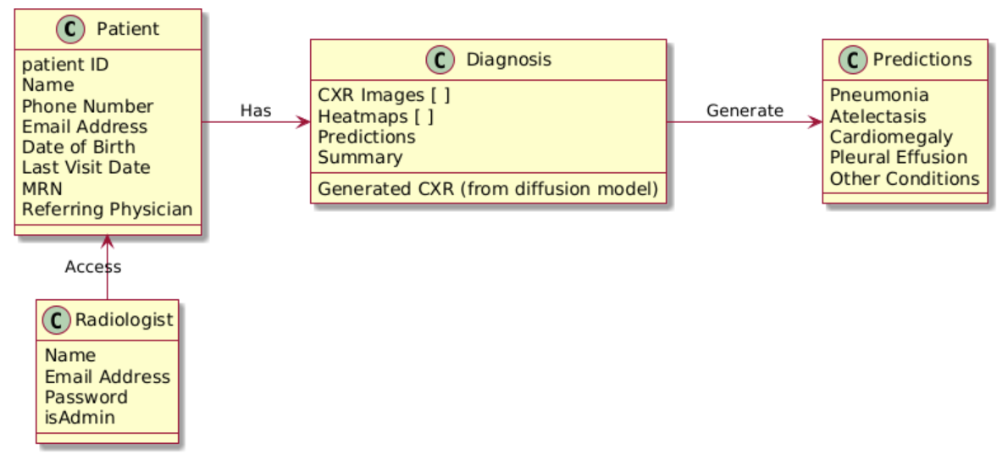
\includegraphics[width=0.8\textwidth]{images/bussiness_data_model.png}
    \caption{Business Data Model}
    \label{fig:business_data_model}
\end{figure}
\subsection{Data Dictionary}
\begin{itemize}
    \item \textbf{Patient}: contains all the relevant personal details of the patient, accessed via the database of patients.

    \item \textbf{Radiologist}: contains authentication details and access level for the users that can access the system.

    \item \textbf{Diagnosis}: Diagnostic data from chest X-ray analysis.
    \begin{itemize}
        \item \textbf{CXR Images}: Uploaded chest X-rays.
        \item \textbf{Heatmaps}: Attention maps from X-rays.
        \item \textbf{Predictions}: Probability scores for various conditions.
        \item \textbf{Summary}: Brief diagnostic overview.
        \item \textbf{Generated CXR}: Simulated X-rays from diffusion models.
    \end{itemize}

    \item \textbf{Predictions}: contains all prediction/risk values for the diseases considered.
\end{itemize}

\section{The Scope of the Product}

\textbf{Current Content:} Defines the general functionality of the AI tool. \\
\\
\textbf{\textcolor{blue}{Update Needed:}} Shift focus to \textbf{classification performance} rather than diagnostic report generation. Ensure \textbf{multi-class classification output with confidence scores} is emphasized.

\subsection{Product Boundary}
The system covers the Automated Chest X-ray Diagnosis lifecycle, from image input to diagnostic report generation using diffusion models. It focuses on detecting lung-related conditions like pneumonia and pleural effusion. Key components include image analysis, disease prediction through diffusion models, a web interface for radiologists, and security for patient data. The application excludes real-time consultations and other imaging types.

\subsection{Product Use Case Table}
The following table summarizes the product use cases for the project's proposed solution:

\begin{table}[h!]
    \centering
    \caption{Product Use Case Table}
    \begin{tabular}{|c|p{12cm}|}
        \hline
        \textbf{Use Case ID} & \textbf{Use Case Summary} \\
        \hline
        PUC1 & Process chest X-ray image using diffusion model \\
        \hline
        PUC2 & Generate disease predictions from processed X-ray \\
        \hline
        PUC3 & Convert predictions into a structured diagnostic report \\
        \hline
        PUC4 & Display the diagnostic findings on the web interface \\
        \hline
        PUC5 & Generate synthetic CXR images for disease analysis \\
        \hline
    \end{tabular}
\end{table}
\subsection{Individual Product Use Cases (PUC's)}
The following are the individual product use cases (PUCs), with a description, lists of actors, preconditions, and postconditions provided for each.

\begin{itemize}
    \item 
    \begin{description}
        \item[Description:] The system takes a chest X-ray image as input and processes it using diffusion models to identify abnormalities.
        \item[Actors:] Diffusion model, chest X-ray image.
        \item[Precondition(s):] Valid chest X-ray image input is provided.
        \item[Postcondition(s):] Processed image with identified abnormalities is generated.
    \end{description}
    
    \item 
    \begin{description}
        \item[Description:] The system generates a comprehensive list of disease predictions based on the processed chest X-ray image.
        \item[Actors:] Diffusion model, disease prediction module.
        \item[Precondition(s):] Processed image with identified abnormalities is provided.
        \item[Postcondition(s):] A list of disease predictions is generated.
    \end{description}
    
    \item 
    \begin{description}
        \item[Description:] The system converts the list of disease predictions into a structured diagnostic report for healthcare professionals.
        \item[Actors:] Prediction list, report generation module.
        \item[Precondition(s):] A list of disease predictions is provided.
        \item[Postcondition(s):] A diagnostic report is generated.
    \end{description}
    
    \item 
    \begin{description}
        \item[Description:] The user interface module displays the diagnostic report for the radiologist or physician.
        \item[Actors:] User interface module, radiologist/physician.
        \item[Precondition(s):] Diagnostic report is provided.
        \item[Postcondition(s):] Diagnostic report is displayed on the web interface.
    \end{description}
    
    \item 
    \begin{description}
        \item[Description:] The system generates synthetic CXR images with specific disease signatures for analysis and training purposes.
        \item[Actors:] Diffusion model, chest X-ray image.
        \item[Precondition(s):] Valid chest X-ray image input is provided.
        \item[Postcondition(s):] Synthetic CXR images with disease signatures are generated.
    \end{description}
\end{itemize}

\section{Functional Requirements}

\textbf{Current Content:} The system is designed for disease identification and report generation. \\
\\
\textbf{\textcolor{blue}{Update Needed:}}
\begin{itemize}
    \item Define the \textbf{specific disease categories} that the model will classify, ensuring clarity on the scope of detection.
    \item Introduce a requirement for \textbf{heatmap visualization (e.g., Grad-CAM)} to provide explainability in classifications.
    \item Shift the reporting format from \textbf{free-form medical reports} to \textbf{structured classification outputs}, including \textbf{disease type, confidence scores, and severity indicators}.
\end{itemize}\\

\subsection{Functional Requirements}

\begin{itemize}
    \item \textbf{FR1: The system shall accept and read CXR (Chest X-ray) images as input.}
    \begin{itemize}
        \item \textbf{Rationale:} This is the primary input to the diffusion model for disease signature generation.
        \item \textbf{Fit Criterion:} The system can successfully process CXR images and recognize valid formats.
        \item \textbf{Product Use Case(s):} PUC1
    \end{itemize}
    
    \item \textbf{FR2: The system shall process CXR images using a diffusion model to generate disease signatures at specified locations.}
    \begin{itemize}
        \item \textbf{Rationale:} This model allows the system to modify the original image by adding disease-specific patterns for diagnosis.
        \item \textbf{Fit Criterion:} The system generates an output image with added disease signatures based on user-defined specifications.
        \item \textbf{Product Use Case(s):} PUC1, PUC2
    \end{itemize}
    
    \item \textbf{FR3: The system shall identify and classify multiple diseases in the CXR image, including (but not limited to) Pneumonia, Atelectasis, Cardiomegaly, and Pleural Effusion.}
    \begin{itemize}
        \item \textbf{Rationale:} The goal is to detect and classify common lung and cardiac conditions.
        \item \textbf{Fit Criterion:} The system detects the presence or absence of diseases with an accuracy greater than 90\% for each disease.
        \item \textbf{Product Use Case(s):} PUC2, PUC5
    \end{itemize}
    
    \item \textbf{FR4: The system shall generate a structured diagnostic report from the findings on the CXR image.}
    \begin{itemize}
        \item \textbf{Rationale:} Medical professionals need a clear report outlining the findings and severity of the conditions detected.
        \item \textbf{Fit Criterion:} The system generates a report detailing the diseases, their severity, and the locations in the image where the abnormalities were detected.
        \item \textbf{Product Use Case(s):} PUC3, PUC4
    \end{itemize}
    
    \item \textbf{FR5: The system shall display heatmaps on the CXR images to indicate the locations of the detected disease signatures.}
    \begin{itemize}
        \item \textbf{Rationale:} The heatmaps assist radiologists in pinpointing the areas of concern for further analysis.
        \item \textbf{Fit Criterion:} The system overlays heatmaps on the CXR images and accurately highlights regions where disease signatures are present.
        \item \textbf{Product Use Case(s):} PUC5
    \end{itemize}
    
    \item \textbf{FR6: The system shall allow users to access the diagnostic reports and heatmaps via a web-based user interface.}
    \begin{itemize}
        \item \textbf{Rationale:} Medical professionals need to access diagnostic results remotely and conveniently.
        \item \textbf{Fit Criterion:} The system successfully displays diagnostic reports and heatmaps on the web interface for authorized users.
        \item \textbf{Product Use Case(s):} PUC4
    \end{itemize}
    
    \item \textbf{FR7: The system shall store patient data, CXR images, and diagnostic reports securely in a backend database.}
    \begin{itemize}
        \item \textbf{Rationale:} Patient confidentiality and secure storage are essential for medical data.
        \item \textbf{Fit Criterion:} The system successfully stores and retrieves CXR images, diagnostic reports, and patient information in a secure database.
        \item \textbf{Product Use Case(s):} PUC1, PUC4
    \end{itemize}
    
    \item \textbf{FR8: The system shall provide authentication and authorization mechanisms to control access to the system.}
    \begin{itemize}
        \item \textbf{Rationale:} Only authorized medical professionals should be able to access the system and patient data.
        \item \textbf{Fit Criterion:} The system requires valid login credentials for access and restricts actions based on user roles.
        \item \textbf{Product Use Case(s):} PUC1, PUC4
    \end{itemize}
\end{itemize}

\section{Look and Feel Requirements}

\textbf{Current Content:} Covers user interface aesthetics. \\
\\
\textbf{\textcolor{blue}{Update Needed:}} Define \textbf{visualization tools such as heatmaps (Grad-CAM)} for classification transparency. Ensure UI allows \textbf{clear distinction of multi-class predictions}.

\subsection{Appearance Requirements}
NF-AR1 The web app will incorporate a cool, and calming color scheme that combines white and soft 
tones of blue.

Rationale: This color scheme is associated with healthcare environments and can ease user’s 
anxiety while building a sense of confidence and trust in the software.

Fit Criterion: User surveys indicate that at least 75\% of users feel the color scheme contributes 
positively to their experience.

\subsection{Style Requirements}
NF-SR1 The web app will have a consistent simple style that makes it easy to use and experiment 
with the model, without adding unnecessary complexity.

Rationale: Keeping the style simple and uniform will help users focus on using the diffusion model 
without getting distracted design elements. This is because the web app serves to be exclusively 
used to experiment with the model, and its results. 
\\\\
NF-SR2: The software interface shall maintain a clean and organized aesthetic.

Rationale: A clutter-free interface will enhance user focus, provides a professional appearance 
and enables more effective use of the software.

Fit Criterion: Usability tests should reveal that 80\% of users find the interface easy to 
navigate without feeling overwhelmed.

\section{Usability and Humanity Requirements}

\textbf{Current Content:} Describes usability for medical professionals. \\
\\
\textbf{\textcolor{blue}{Update Needed:}} Emphasize \textbf{ease of interpreting multi-class classification results}. Ensure \textbf{clear explanations for ambiguous or uncertain classifications}.

\subsection{Ease of Use Requirements}
NF-EUR0 The web app should focus only on core functionality, with no extra features that might 
confuse users.

Rationale: The simpler the app, the easier it will be for users to focus on generating chest X-ray 
images without getting lost in unnecessary options.

Fit Criterion: Testers should be able to perform basic tasks, like generating an image, without 
needing extra guidance, and no irrelevant features should be present.

Traceability: Traces to functional requirements related to user interface simplicity and task 
completion.
\\\\
NF-EU2: The software shall be intuitive enough that users can remember how to operate it after 1-2 
training sessions.

Rationale: Ease of remembering ensures that even occasional users can operate it effectively 
without needing extensive retraining. This simplicity is crucial, especially since it will be used 
daily.

Fit Criterion: One month after training, 80\% of users shall report they can navigate the software 
and perform basic functions without assistance.
\subsection{Personalization and Internationalization Requirements}
N/A

\subsection{Learning Requirements}
NF-LR0 The web app should be easy to learn, allowing users to quickly understand how to use it 
without needing tutorials or training.

Rationale: Since this is a research-focused tool, we want users (who may be students, researchers, 
or radiologists) to get hands-on with the model right away without wasting time on complex 
instructions.

Fit Criterion: Users should be able to generate an image within the first minute of using the app, even without prior experience.

\subsection{Understandability and Politeness Requirements}
NF-UPR0 The chest X-ray images generated by the diffusion model should closely resemble real-world 
X-rays used in hospitals.

Rationale: The generated images must be realistic and meet a standard that could be accepted by 
radiologists for them to be useful in a medical or research context.

Fit Criterion: Radiologists or other medical professionals should not be able to easily 
distinguish between the generated X-rays and real-world X-rays after reviewing them.

\subsection{Accessibility Requirements}
N/A

\section{Performance Requirements}

\textbf{Current Content:} Focuses on processing speed and reliability. \\
\\
\textbf{\textcolor{blue}{Update Needed:}} Define metrics such as \textbf{classification latency (time taken to process X-rays), model accuracy per disease category, and system robustness against adversarial inputs}.

\subsection{Speed and Latency Requirements}
NF-SLR0 The system should generate a chest X-ray image within a reasonable amount of time after a 
request is made.

Rationale: Since the model is generating images based on complex diffusion processes, it should 
still be fast enough to keep users engaged. It should likewise include a loading indicator such 
that the user can interpret how long of a wait there is.

Fit Criterion: A chest X-ray image is generated within 1 minute of the user request.

\subsection{Safety-Critical Requirements}
NF-SCR0 The system should not store or process any personal data unrelated to the generation of 
chest X-ray images.

Rationale: This is a research tool meant to generate synthetic images, so there’s no need for 
sensitive or personal data to be collected.

Fit Criterion: Only data related to image generation (e.g., input parameters) will be processed or 
stored.

\subsection{Precision or Accuracy Requirements}
NF-PAR0 The generated chest X-ray images should be visually similar to real medical chest X-rays.

Rationale: The images generated by the diffusion model need to be realistic so that they could 
potentially be useful in medical or research settings.

Fit Criterion: At least 90\% of medical professionals surveyed should agree that the generated 
images closely resemble real chest X-rays.

\subsection{Robustness or Fault-Tolerance Requirements}
NF-RFTR0 The system should be stable and available for use most of the time.

Rationale: Since users will be experimenting with the model, it needs to be reliable and not crash 
frequently. This would otherwise deter users from experimenting with the mode.

Fit Criterion: The system should be available at least 99\% of the time, with minimal downtime (no 
more than 1 hour of downtime per week).


\subsection{Capacity Requirements}
NF-CR0 The system should only generate one chest X-ray image at a time.

Rationale: Generating a diffusion-based chest X-ray image requires significant processing power 
and time, so the system should focus on producing a single, high-quality image per request.

Fit Criterion: The system will only allow for one image to be generated at a time, with no 
simultaneous image requests.

\subsection{Scalability or Extensibility Requirements}
NF-SER0 The system will be maintained to ensure it continues functioning properly with updates to 
the diffusion model but will not include new features beyond its MVP scope.

Rationale: As an MVP, the system is designed to showcase the core diffusion model. While updates
 to the model will be accommodated, no new features will be added.

Fit Criterion: The system should remain operational and compatible with any future changes to the
 diffusion model, without requiring major redesigns or additional functionality.

\subsection{Longevity Requirements}
NF-LR0 The system should be designed to remain operational and reliable for at least 3 years after 
the initial deployment, or as long as the model and technology is relevant, with minimal 
maintenance required.

Rationale: Since the system is an MVP for research purposes, it should be able to function long 
enough for ongoing experiments and potential further development without requiring constant 
updates or significant maintenance. However, if diffusion models are no longer useful or are no 
longer a research endeavour, the project will more prematurely close.

Fit Criterion: The system should function without major failures or the need for large-scale 
updates for at least 3 years, as long as the server infrastructure and diffusion model research 
remain stable.


\section{Operational and Environmental Requirements}

\textbf{Current Content:} Describes deployment environment. \\
\\
\textbf{\textcolor{blue}{Update Needed:}} Ensure system is \textbf{optimized for cloud deployment} and compatible with \textbf{hospital IT infrastructure (PACS, EHRs)}.

\subsection{Expected Physical Environment}
NF-EPE0 The web app will be accessed through regular computers or mobile devices with internet 
access. Physical location is irrelevant.

Rationale: Since this is an MVP for research purposes, users (such as students, researchers, and 
radiologists) will interact with the system from their usual devices, requiring nothing beyond an 
internet connection.

Fit Criterion: N/A

\subsection{Wider Environment Requirements}
N/A


\subsection{Requirements for Interfacing with Adjacent Systems}
NF-RIAS0 The system will be self-contained, requiring no external systems or servers to function, 
outside of infrastructure such as web-hosting provided by cloud services.

Rationale: Since this is an MVP for experimenting with the diffusion model, the system only needs
 to handle the model itself without interacting with other medical systems or databases.

Fit Criterion: The system should function independently and generate images without requiring 
integration with any third-party systems.

\subsection{Productization Requirements}
NF-PR0 The system will be accessible via a simple web interface and will only require a stable 
internet connection.

Rationale: The system needs to be easy for users to access from anywhere using their browser, 
without needing to install any additional software.

Fit Criterion: The system should be accessible and fully functional as long as the user has a 
stable internet connection.

\subsection{Release Requirements}
N/A

\section{Maintainability and Support Requirements}

\textbf{Current Content:} Covers updates and long-term maintenance. \\
\\
\textbf{\textcolor{blue}{Update Needed:}} Define \textbf{requirements for periodic model retraining} with \textbf{new datasets} to improve accuracy and prevent model drift.

\subsection{Maintenance Requirements}
NF-MR0 The system will be maintained by the developers to ensure it stays operational and 
compatible with updates to the diffusion model.

Rationale: Since this is an MVP, the primary focus is on keeping the system working as the 
diffusion model is improved or adjusted. No external support teams are needed as it will be 
managed by the project team.

Fit Criterion: The developers can make updates or fixes as needed to keep the system operational.

\subsection{Supportability Requirements}
NF-SR0 The system will be self-sufficient, with all necessary documentation provided so that users 
can understand how to experiment with the diffusion model.

Rationale: The web app should include simple documentation or guidelines to help users experiment
 with the model on their own, minimizing the need for external support.

Fit Criterion: Users can access the documentation and experiment with the model without needing 
further assistance.

\subsection{Adaptability Requirements}
N/A

\section{Security Requirements}

\textbf{Current Content:} Focuses on basic security measures. \\
\\
\textbf{\textcolor{blue}{Update Needed:}} Expand to include \textbf{data encryption, access control for medical professionals, and compliance with HIPAA and GDPR} for handling patient data.

\subsection{Access Requirements}
NF-AR0 The web app will be publicly accessible to anyone, without the need for login or 
credentials.

Rationale: The purpose of the web app is to allow anyone reading the research paper to easily 
access and experiment with the diffusion model, so no user restrictions are necessary.

Fit Criterion: The web app can be accessed by anyone without needing to sign in or provide any 
credentials.

\subsection{Integrity Requirements}
NF-IR0 The web app will output the generated chest X-ray image as produced by the diffusion model 
without further data protection or tampering restrictions.

Rationale: The main purpose of the web app is to allow users to experiment with the model and view 
the generated images discussed in the associated research paper. What users do with the images 
afterward is beyond the scope of the system’s responsibility.

Fit Criterion: The web app successfully outputs the generated image without further concern for 
data protection after it is delivered to the user.


\subsection{Privacy Requirements}
NF-PR0 The system will not collect any personal data from users interacting with the web app.

Rationale: Since the system is intended for public experimentation, there is no need to collect 
personal information or track users’ activities.

Fit Criterion: The web app does not request or store any personal information from users during 
their interactions with the system.

\subsection{Audit Requirements}
NF-AR0 The system will not require any formal security audits as it is a public web app designed 
for experimentation only.

Rationale: Since this is an MVP for public use with no sensitive data involved, regular security 
audits are unnecessary.

Fit Criterion: N/A

\subsection{Immunity Requirements}
N/A

\section{Cultural Requirements}

\textbf{Current Content:} Mentions accessibility and language support. \\
\\
\textbf{\textcolor{blue}{Update Needed:}} Ensure \textbf{multi-language support for model outputs} and adaptability for \textbf{different healthcare regions and regulatory environments}.

\subsection{Cultural Requirements}
NF-CR0 The web app will be usable by people from any background or culture with no restrictions 
such as in region. However it will be written in English, but users can rely on modern web 
browsers to translate it into other languages if needed.

Rationale: The research and thus the web app should be able to be explored by anyone who is 
interested in the findings. English is the most universally understood language, making it 
accessible to a large audience. However, users who prefer other languages can easily use browser 
translation tools.

Fit Criterion: The web app is fully functional in English, and users are able to translate it into 
other languages using their browser if necessary.


\section{Compliance Requirements}

\textbf{Current Content:} Lists general compliance needs. \\
\\
\textbf{\textcolor{blue}{Update Needed:}} Expand to include \textbf{FDA and CE regulatory compliance} for AI-based medical classification tools.

\subsection{Legal Requirements}
NF-LR0 The web app will comply with general data privacy laws by ensuring that no personal or 
sensitive data is collected.

Rationale: As the web app is for public experimentation with no personal information involved, it 
should comply with privacy laws by not collecting user data.

Fit Criterion: The web app will not store or request any personal information from users.

\subsection{Standards Compliance Requirements}
NF-SCR0 The chest X-ray images produced by the diffusion model must meet the standards of 
real-world chest X-rays used in radiology.

Rationale: While the web app is for experimentation and exploring the research findings, the 
images generated by the diffusion model must still comply with radiology standards to be viable 
for training models and potential real-world use.

Fit Criterion: The generated chest X-rays meet the quality and standards of actual medical chest 
X-rays used in radiology.

\section{Open Issues}
\begin{itemize}
    \item Data Privacy and Security: Implementation of security measures in order to protect 
    patient information. The data stored should be encrypted and anonymized.
    \item Neural Network Optimization: Accurate models are often large and take a long time to 
    produce output. The performance of the algorithms needs to be optimized in order for the model 
    to be usable for chest x-ray analysis.
    \item Web Application Concurrent Requests: The interface to use the neural network is a web 
    application. There may be multiple instances of the web application from different users to 
    access the same neural network in the backend. It will be difficult to make the model support 
    multiple concurrent users.
    \item Explanation of Disease: Making the model explain why it identifies a disease at a 
    specific location will help transparency and let radiologists make a more informed decision on 
    whether to trust it or if it is a false positive.
\end{itemize}

\section{Off-the-Shelf Solutions}
\subsection{Ready-Made Products}
\begin{itemize}
    \item Pretrained Models: There exists pretrained diffusion models that can generate object 
    images. However, many of them are not specialized in generating chest x-ray images with a 
    specific disease at a specific location. By leveraging these existing pretrained models, we 
    can build on top of their neural networks and improve on it to accelerate development.
    \item Chest X-ray Images Dataset: Established collections of chest x-ray images annotated with 
    radiologist’s report will be used to train the neural network. They need to be used because we 
    have no other source of chest x-ray images.
\end{itemize}
\subsection{Reusable Components}
N/A 

\subsection{Products That Can Be Copied}
No products will be copied in place for this project. There are no projects to copy off of since 
this project consists of a research component that will try to improve on existing implementations 
of neural networks in the field. However, this project will produce a neural network model which 
can be copied and used elsewhere for anyone following the license rules.


\section{New Problems}

\textbf{Current Content:} Identifies research gaps. \\
\\
\textbf{\textcolor{blue}{Update Needed:}} Highlight issues such as \textbf{handling multi-label cases where multiple diseases coexist in a single X-ray} and \textbf{model biases based on training data imbalances}.

\subsection{Effects on the Current Environment}
\begin{itemize}
    \item Improvements in neural networks and their ability to identify diseases may lead to an 
    over-reliance on it. Doctors may overly trust the output. It could erode human and traditional 
    skills over time. This will leave healthcare providers less prepared if the model fails, is 
    unavailable, or shows a false positive.
    \item Neural networks do not explain their thoughts. It is a black box. There could be reduced 
    accountability when errors occur as it may be unclear whether the machine or the doctor is at 
    fault.
    \item The diffusion model can generate new chest x-ray images which is great for creating more 
    x-ray datasets. This could be used to further train more chest x-ray neural networks which in 
    turn could improve their ability to identify diseases.
\end{itemize}


\subsection{Effects on the Installed Systems}
N/A 

\subsection{Potential User Problems}
\begin{itemize}
    \item Users or doctors may not want to upload chest x-ray images due to privacy concerns.
    \item Users may accidentally upload non chest x-ray images. The neural network model expects 
    an x-ray image and so its output may be unpredictable.
    \item Radiologists may be skeptical that the neural network model works well and will hesitate 
    adopting the technology. Since a diffusion model generates a chest x-ray image that could be 
    used in training other neural networks, radiologists may also be hesitant in using these 
    generated images in their neural networks research.
\end{itemize}

\subsection{Limitations in the Anticipated Implementation Environment That May
Inhibit the New Product}
\begin{itemize}
    \item Neural network models usually expect to process one image at a time. Since there is only 
    one model in the backend of the web application, there will be a queue to use the model. This 
    will hinder the workflow as the processes must be done sequentially.
    \item The web application is the interface to use the model. It requires the user to have an 
    internet connection in order to load the site. If the internet connection is poor, the user 
    may have a hard time uploading the image.
\end{itemize}

\subsection{Follow-Up Problems}
The web application may store uploaded images. If the encryption for the images is stolen or 
cracked, users may have their medical images exposed. This is a security and privacy concern. 
Users may blame the development team for the lack of security.

\section{Tasks}

\subsection{Project Planning}
\begin{table}[H]
    \begin{tabular}{|l|l|}
    \hline
    \textbf{Deliverable}                          & \textbf{Deadline}      \\ \hline
    Team Formed, Project Selected                 & September 18           \\ \hline
    Problem Statement, POC Plan, Development Plan & September 25           \\ \hline
    Requirements Document Revision 0              & October 11             \\ \hline
    Hazard Analysis 0                             & October 20             \\ \hline
    V\&V Plan Revision 0                          & November 3             \\ \hline
    Proof of Concept Demonstration                & November 13-24         \\ \hline
    Design Document Revision 0                    & January 17             \\ \hline
    Revision 0 Demonstration                      & February 5-February 16 \\ \hline
    V\&V Report Revision 0                        & March 6                \\ \hline
    Final Demonstration (Revision 1)              & March 18-March 29      \\ \hline
    EXPO Demonstration                            & April TBD              \\ \hline
    Final Documentation (Revision 1)              & April 4                \\ \hline
    \end{tabular}
\end{table}

\subsection{Planning of the Development Phases}
\begin{enumerate}
    \item {
        Team Formation and Project Setup (September 18)
        \begin{itemize}
            \item Form the project team and contact supervisor
            \item Set up Github repository
        \end{itemize}
    }
    \item {
        Project Planning and Definition (October 11)
        \begin{itemize}
            \item Develop a detailed project roadmap and define the problem and the project’s scope
            \item Identify stakeholders
            \item Write SRS documentation
        \end{itemize}
    }
    \item {
        Research (October)
        \begin{itemize}
            \item Conduct research on diffusion models and their applications in chest x-ray 
            analysis
            \item Explore new and innovative ways to improve on existing applications of detecting 
            diseases in chest x-ray images
            \item Investigate suitable datasets for training the model
            \item Find relevant frameworks and tools to trail the diffusion model
        \end{itemize}
    }
    \item {
        Initial Implementation (November)
        \begin{itemize}
            \item Cleanse training data, so the images can be used to train the model
            \item Write the Hazard Analysis document
        \end{itemize}
    }
    \item {
        Feature Development (December)
        \begin{itemize}
            \item Develop the front and backend of the web application
            \item Have a proof of concept trained model that can generate new images to some degree
            \item Write the Design document revision 0            
        \end{itemize}
    }
    \item {
        Testing (January)
        \begin{itemize}
            \item Continue training and create iterations of the model to improve its accuracy
            \item Evaluate the achievement of project goals
            \item Conduct risk and user-end assessments
            \item Write Verification and Validation report
        \end{itemize}
    }
    \item {
        Finalization
        \begin{itemize}
            \item Present final demonstration and all final project documentation
            \item Prepare for Expo presentation
        \end{itemize}
    }
\end{enumerate}

\section{Migration to the New Product}
\subsection{Requirements for Migration to the New Product}
N/A. There is no migration. The product is developed from the ground up.

\subsection{Data That Has to be Modified or Translated for the New System}
Training data, which includes pairs of chest x-ray images and radiologist reports, must be 
cleansed so that they can be inputted into the neural network to be trained. Cleansing data could 
involve converting its file type, modifying the images’ shape, and parsing radiologist reports for 
specific words.

\section{Costs}
There are no monetary costs anticipated. All model training will be done locally, so there will be 
no cloud service provider costs. The web application will be hosted locally as well. Should there 
be any costs, the total will not exceed \$500.

\section{User Documentation and Training}

\textbf{Current Content:} Covers basic user guides. \\
\\
\textbf{\textcolor{blue}{Update Needed:}} Ensure documentation includes \textbf{interpretation guides for multi-class classification outputs} and training for \textbf{understanding heatmaps and uncertainty scores}.

\subsection{User Documentation Requirements}
\begin{itemize}
    \item \textbf{User Interface Guide:} A step-by-step guide explaining how users (e.g., 
    radiologists, clinicians) will interact with the web app. This might include:
    \begin{itemize}
        \item How to upload CXR images.
        \item How to interpret the generated diagnostic report.
        \item Understanding heatmaps and disease predictions.
    \end{itemize}
    \item \textbf{System Overview:} A high-level description of how the system works from a user’s 
    perspective.
    \item \textbf{Frequently Asked Questions (FAQ):} A list of common issues users may encounter 
    and how to resolve them.
\end{itemize}

\subsection{Training Requirements}
\begin{itemize}
    \item \textbf{Minimal Training:} Since the system is user-friendly and mostly automated, 
    minimal training is required.
    \item \textbf{Tutorial Session:} A 1-2 hour training session for medical professionals, 
    focusing on:
    \begin{itemize}
        \item How to use the web application.
        \item How to interpret diagnostic reports and heatmaps.
    \end{itemize}
    \item \textbf{Online Help:} Interactive tutorials or video guides embedded in the system.
\end{itemize}


\section{Ideas for Solution}
Potential system improvements and future enhancements:
\begin{itemize}
    \item \textbf{Batch Processing:} Allow processing of multiple CXR images simultaneously for 
    high-volume diagnosis.
    \item \textbf{More Disease Detection:} Add support for additional diseases.
    \item \textbf{Mobile App:} Develop a mobile version for on-the-go use.
    \item \textbf{Advanced AI Models:} Integrate other AI techniques (e.g., GANs, transformers) 
    for better accuracy.
    \item \textbf{EHR Integration:} Connect with electronic health record systems for automatic 
    data exchange.
    \item \textbf{Explainability:} Add AI explanations for predictions to improve transparency.
\end{itemize}

\section{Waiting Room}
Possible future features or enhancements:
\begin{itemize}
    \item \textbf{Batch Processing:} Enable uploading and processing of multiple CXR images.
    \item \textbf{Additional Disease Detection:} Extend the system to identify more conditions.
    \item \textbf{Mobile App:} Consider developing a mobile version for accessibility.
    \item \textbf{Explainability:} Provide AI explanations for the model's predictions.
\end{itemize}



\newpage{}
\section*{Appendix --- Reflection}

\textbf{Current Content:} Summarizes challenges and lessons learned. \\
\\
\textbf{\textcolor{blue}{Update Needed:}} Expand reflections on \textbf{handling data bias, tuning hyperparameters for optimal classification, and challenges in model interpretability}.


The information in this section will be used to evaluate the team members on the
graduate attribute of Lifelong Learning.  Please answer the following questions:

\begin{enumerate}
  \item What knowledge and skills will the team collectively need to acquire to
  successfully complete this capstone project?  Examples of possible knowledge
  to acquire include domain specific knowledge from the domain of your
  application, or software engineering knowledge, mechatronics knowledge or
  computer science knowledge.  Skills may be related to technology, or writing,
  or presentation, or team management, etc.  You should look to identify at
  least one item for each team member.

  To successfully complete the chest x-ray disease identification and image generation project, 
  the team must learn a diverse set of knowledge and skills. The AI/ML developer must be 
  proficient in machine learning techniques. They should especially be knowledgeable in diffusion 
  models and computer vision, and use libraries like PyTorch to build the neural network. They 
  should also understand parameter tuning to enhance model accuracy. A data scientist will focus 
  on data preprocessing and augmentation to increase the training dataset’s variety. Their skills 
  in handling large datasets and using tools like Pandas and NumPy for exploratory analysis are 
  important. The frontend developer should know web development frameworks like React to build an 
  intuitive interface where users can upload x-ray images and view the model’s predictions. The 
  backend developer will need expertise in hosting services locally to run the AI model for the 
  web application. They will ensure it integrates smoothly with the web application. Lastly, the 
  project manager must have strong team management skills. They will ensure the team meets 
  milestones and communicates clearly with stakeholders through presentations and reports. Each 
  team member must combine their technical expertise with effective collaboration to finish the 
  project.

  \item For each of the knowledge areas and skills identified in the previous
  question, what are at least two approaches to acquiring the knowledge or
  mastering the skill?  Of the identified approaches, which will each team
  member pursue, and why did they make this choice?

  To learn the necessary knowledge and skills for the project, team members have several 
  approaches. The AI/ML developer can either complete specialized online courses like Coursera’s 
  deep learning series or review notes from SFWRENG 4ML3 machine learning course. Online courses 
  offers more flexibility learning diffusion models at their own pace. The data scientist can 
  improve their skills through looking at Kaggle projects. Many Kaggle competitions have projects 
  where other people tried to cleanse data from different datasets. The data scientist can 
  practice and follow in their Github’s footsteps to learn from the community. The frontend 
  developer could learn from Youtube tutorials and documentation for frameworks like React. With 
  self-paced tutorials, they can quickly apply their learning in building the interface. The 
  backend developer can either take cloud certifications from AWS or practice hosting a home 
  server which they can connect to at home. A home server is great for learning about networks and 
  how to connect to them. It also gives them options to run whatever service they want. Lastly, 
  the project manager can read project management books like Scrum: The Art of Doing Twice the 
  Work in Half the Time. They could also go outside and talk to people to learn how to communicate 
  normally with others in a professional manner.

\end{enumerate}

\end{document}